\chapter{Congruencia}

%----------definición 4.1
\begin{tcolorbox}[colframe=white]
    \begin{def.}
	dos segmentos son congruentes si tienen la misma longitud. dos ángulos son congruentes si tiene igual medida.\\\\
	como $\overline{ab}=\overline{cd} \quad \rightarrow \quad ab$ es congruente con $cd$.\\\\
	si $\alpha = \beta \quad \rightarrow \quad a\widehat{o}b$ es congruente con $a^{'}\widehat{o^{'}}b^{'}$\\\\
    \end{def.}
\end{tcolorbox}

%----------definición 4.1
\begin{tcolorbox}[colframe=white]
    \begin{def.}
	Dos triángulos son congruentes si fuese posible establecer una correspondencia biunívoca entre sus vértices tal que los lados y ángulos correspondientes sean congruentes.
    \end{def.}
\end{tcolorbox}

%----------axioma 4.1
\begin{tcolorbox}[colframe=white]
    \begin{axioma}[Lado ángulo lado (LAL)]
	Dados los triángulos $ABC$ y $EFG$, si $AB=EF, \; AC=EG,\; \widehat{A}=\widehat{E}$ entonces $EFG$. 
    \end{axioma}
\end{tcolorbox}

    %----------teorema 4.1
    \begin{teo}[Ángulo lado angulo (ALA)] Dados $ABC$ y $EFG$ si $AB=EF, \; \widehat{A}=\widehat{E} \widehat{B}=\widehat{F}$ entonces $DEF$.
	Demostración.-\; Sean $ABC$ y $EFG$ tal que, $AB=EF$, $\widehat{A}=\widehat{E}$ y $\widehat{B}=\widehat{F}$. Sea $D$ en $S_{AC}$ tal que $AD=EG$. Luego, por el axioma 4.1, $DAB=GEB$. Así, $A\widehat{B}D=\widehat{F},$ 
    \end{teo}

%----------definición 4.2
\begin{tcolorbox}[colframe=white]
    \begin{def.}
	Un triángulo se dice isósceles si tiene dos lados congruentes.
    \end{def.}
\end{tcolorbox}

    %----------proposición 4.1
    \begin{proposicion}
	En un triángulo isósceles los ángulos de la base son congruentes.\\\\
	    Demostración.-\;
    \end{proposicion}

    %----------proposición 4.1
    \begin{proposicion}
	Si en un triángulo $ABC$, se tienen dos ángulos congruentes, entonces el triángulo es isósceles.\\\\
	    Demostración.-\;
    \end{proposicion}

%----------definición 4.2
\begin{tcolorbox}[colframe=white]
    \begin{def.}
	Sea $ABC$ un triángulo y $D$ un punto en la recta $BC$. La mediana del triángulo relativa al vértice  $A$ y lado $BC$, (va de $A$ hasta $BC$) es el segmento que une $A$ con $D$ el punto medio de $BC$. El segmento $AD$ se llama bisectriz de $\widehat{A}$ si $S_{AD}$ divide al ángulo en $A$ en dos ángulos congruentes. El segmento $AD$ se llama altura del triángulo relativa al vértice $A$ y lado $BC$ si $AD$ es perpendicular a la recta $BC$. Si $AD$ es altura entonces $BC$ se dice base.
    \end{def.}
\end{tcolorbox}

    %----------proposición 4.1
    \begin{proposicion}
	En un triángulo isósceles la mediana relativa a la base es también bisectriz y altura.\\\\
	    Demostración.-\;
    \end{proposicion}

    %----------teorema 4.2
    \begin{teo}[Criterio (LLL) de congruencia] Si dos triángulos tienen tres lados correspondientes congruentes, entonces los triángulos son congruentes.
	Demostración.-\;
    \end{teo}

\section{Ejercicios}

\begin{enumerate}[\Large\bfseries 1.]

	%--------------------1.
	\item En la figura, los ángulos $\alpha$ y $\beta$ son iguales. Muestre que $AC=BC$\\

	\begin{center}
	    \begin{tikzpicture}
		\draw(0,0)node[left]{$C$}--(5,1.5)node[above]{$A$}; 
		\draw(0,0)--(5,-1.5)node[below]{$B$}; 
		\draw(4.2,-1.25)--(4.2,1.25);
		\draw [color=black](12:5cm) node[rotate=0] {$\alpha$};
		\draw [red!50!black,very thick](11:4.27cm) arc (-90:20:.4cm);
		\draw [color=black](-12:5cm) node[rotate=0] {$\beta$};
		\draw [red!50!black,very thick](-17:4.8cm) arc (-20:90:.4cm);
	    \end{tikzpicture}
	\end{center}
    
	Demostración.-\; Considere la figura anterior y observe que $\alpha$ es el suplemento $B\widehat{A}C$ y $\beta$ es el suplemento $A\widehat{B}C$, entonces: $\alpha + ABC = 180^{\circ}\,\,\, e \,\,\, \beta + ABC = 180^{\circ}$ haciendo $\alpha = 180^{\circ} - B\widehat{A}C$ y $\beta = 180^{\circ} - A\widehat{B}C$, cómo $\alpha = \beta$ tenemos $180^{\circ} - B\widehat{A}C = 180^{\circ} - A\widehat{B}C$ entonces $B\widehat{A}C=A\widehat{B}C$\\
	Como todo triángulo isósceles tiene ángulos de base congruentes y viceversa, queda demostrado.\\\\

	%--------------------2.
	\item En la figura, se tiene $AB=AC$ y $BD=CE$. Muestre que.

	\begin{center}
	    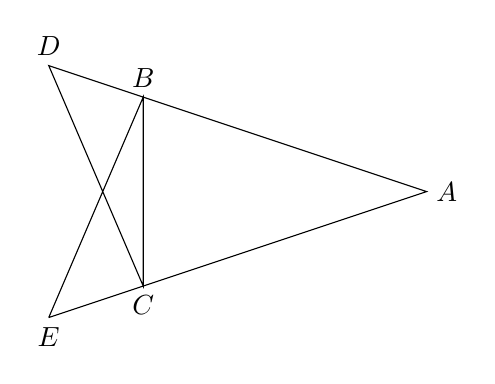
\begin{tikzpicture}[scale=.8]
		\draw(0,0)node[below]{$E$}--(6,2)node[right]{$A$}--(0,4)node[above]{$D$}--(1.5,.5)node[below]{$C$}--(1.5,3.5)node[above]{$B$}--(0,0);
	    \end{tikzpicture}
	\end{center}

	\begin{enumerate}[\bfseries a)]

	    %----------a)
	    \item $ACD=ABE$\\\\
	    Demostración.-\; Por hipótesis $AB = AC$ luego $\triangle ABC$ isósceles y ángulos $A\widehat{B}C$ y $A\widehat{C}B$. Como $\triangle DBC$ y $\triangle ECB$ comparten el lado $BC$ y por hipótesis $BD = EC$ en el caso $LAL \triangle DBC$ y congruente con $\triangle ECB$ lo que implica, $C\widehat{B}E = B\widehat{C}D$ así:
	    $$A\widehat{C}D = A\widehat{B}C + C \widehat{B}E = A\widehat{C}B + B\widehat{C} D = A\widehat{B}E$$
	    $$ACD=ABE$$\\\\

	    %----------b)
	    \item $BCD=CBE$\\\\
	    Demostración.-\; Podemos demostrar similar a la parte $a)$\\\\

	\end{enumerate}

	%--------------------3. 
	\item En la figura, $AC=AD$ y $AB$ es la bisectriz del ángulo $C\widehat{A}D$. Pruebe que los triángulos $ACB$ y $ADB$ son congruentes.
	\begin{center}
	    \begin{tikzpicture}
		\draw(0,0)node[left]{$A$}--(4,-2)node[below]{$D$}--(6,0)node[right]{$B$}--(4,2)node[above]{$C$}--(0,0)--(6,0);
	    \end{tikzpicture}
	\end{center}

	Demostración.-\; Si $AB$ es bisectriz de $CAD$ entonces $CAB = BAD$. Como $CA = AD$ y $AB$ es común tanto para $\triangle ADB$ como para $\triangle CAB$, entonces, en el caso $LAL$, $\triangle ACB = \triangle ADB$.\\\\

	%--------------------4.
	\item En la figura, el punto $A$ es el punto medio de los segmentos $CB$ y $DE$. Pruebe que los triángulos $ABD$ y $ACE$ son congruentes.
	\begin{center}
	    \begin{tikzpicture}
		\draw(0,0)node[left]{$D$}--(7,0)node[right]{$E$}--(5.5,1.5)node[above]{$C$}--(1.5,-1.5)node[below]{$B$}--(0,0);
		\draw(3.5,0)node[above]{$A$};
	    \end{tikzpicture}
	\end{center}

	Demostración.-\; Los ángulos $C\widehat{A}E = D\widehat{A}B$ porque son opuestos por el vértice. En cuanto a la hipótesis $CA = BA$ y $DA = AE$ para el caso $LAL$, $\triangle ABD = \triangle ACE$.\\\\

	%--------------------5.
	\item En la figura, los ángulos $\widehat{A}$ y $\widehat{C}$ son rectos y el segmento $DE$ corta $CA$ en el punto medio $B$ de $CA$. Muestre que $DA=CE$.

	\begin{center}
	    \begin{tikzpicture}
		\draw(0,0)node[left]{$C$}--(7,0)node[right]{$A$}--(5.5,1.5)node[above]{$D$}--(1.5,-1.5)node[below]{$E$}--(0,0);
		\draw(3.5,0)node[above]{$B$};
	    \end{tikzpicture}
	\end{center}

	Demostración.-\; Los ángulos $D\widehat{B}A = C\widehat{B}E$ porque están opuestos por el vértice y como $CA = BA$ por hipótesis, entonces por el caso $ALA$, $\triangle ABD = \triangle CEB$ que implica $DA = CE$.\\\\

	%--------------------6.
	\item En la figura, se sabe que $AC=OB$, $OD=OA$ y $B\widehat{O}D=C\widehat{O}A$. Muestre que $CD=BA.$

	\begin{center}
	    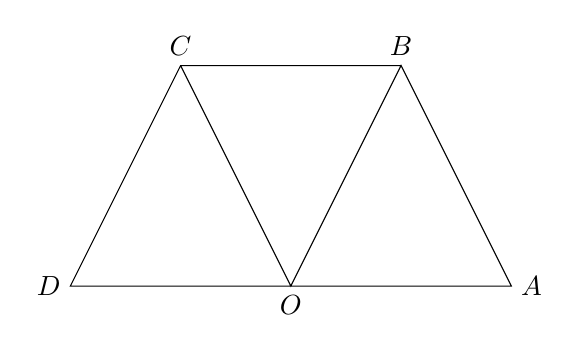
\begin{tikzpicture}[scale=.7]
		\draw(0,0)node[above]{$B$}--(-4,0)node[above]{$C$}--(-6,-4)node[left]{$D$}--(2,-4)node[right]{$A$}--(0,0)--(-2,-4)node[below]{$O$}--(-4,0);
	    \end{tikzpicture}
	\end{center}

	Pro hipótesis $BOD=COA$ con, $$B\widehat{O}D = B\widehat{O}D + C\widehat{O}A = C\widehat{O}D + B\widehat{O}A \,\,\, (1)$$
	y por el esquema $C\widehat{O}B = C\widehat{O}D$, luego por el caso $LAL$, $\triangle BOA = \triangle COD$ que implica $CD = BA$.\\\\

	%--------------------7.
	\item En la figura, $C\widehat{M}A$ es un ángulo recto y $M$ el punto medio de $AB$. Muestre que $CA=CB$.

	\begin{center}
	    \begin{tikzpicture}
		\draw(0,0)--(4,0);
		\draw(3,1.5)node[above]{$A$}--(3,-1.5)node[below]{$B$};
		\filldraw[black](1,0) circle(1.5pt) node[above]{$C$};
		\filldraw[black](3.5,0) node[above]{$M$};
	    \end{tikzpicture}
	\end{center}

	Sea $B\widehat{M}C$ y el suplemento $C\widehat{M}A$, luego $C\widehat{M}A + B\widehat{M}C = 180^{\circ}$. Como $C\widehat{M}A = 90^{\circ}$ tenemos $B\widehat{M}C = 180^{\circ} - 90^{\circ} = 90^{\circ}$, entonces $CMA = BMC$ como $M$ y el punto medio de $AB$, tenemos $AM = MB$. Dado que $CM$ es un lado común de $\triangle AMC$ y $\triangle BMC$ para el caso $LAL$, entonces $\triangle AMC = \triangle BMC$, lo que implica $CA = CB$.\\\\
	
	%--------------------8.
	\item Muestre que, si en un triángulo los tres lados son congruentes, entonces tiene también los tres ángulos congruentes.\\\\
	Demostración.-\; Considere el siguiente gráfico.

	\begin{center}
	    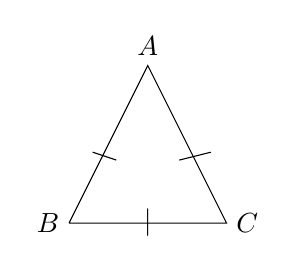
\begin{tikzpicture}
		\draw(0,0)node[left]{$B$}--(2,0)node[right]{$C$}--(1,2)node[above]{$A$}--(0,0);
		\draw(1,0)node[]{$|$};
		\draw(.6,.8)--(.3,.9);
		\draw(1.4,.8)--(1.8,.9);
	    \end{tikzpicture}
	\end{center}

	Si $\triangle ABC$ es equilátero, entonces también es isósceles de la base $BC$ y, por lo tanto, los ángulos de su base serán congruentes, esto es: $\widehat{B} = \widehat{C}$. Ahora, tomando $AB$ como base, por la misma razón tendremos $\widehat{A} = \widehat{C}$, lo que implica $\widehat{A} = \widehat{B} = \widehat{C}$.\\\\

	%--------------------9.
	\item En la figura, $ABD$ y $BCD$ son triángulos isósceles con base $DB$. Pruebe que los ángulos $A\widehat{B}C$ y $A\widehat{D}C$ son congruentes.

	\begin{center}
	    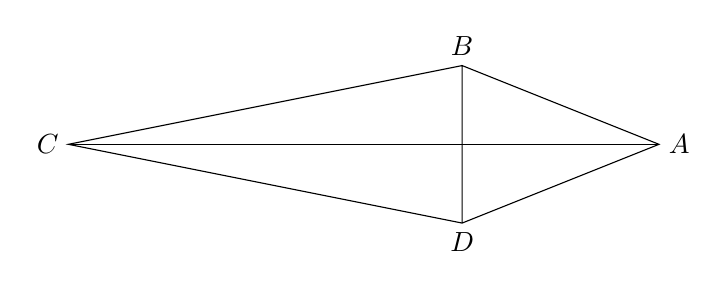
\begin{tikzpicture}
		\draw(0,0)node[below]{$D$}--(0,2)node[above]{$B$}--(2.5,1)node[right]{$A$}--(0,0)--(-5,1)node[left]{$C$}--(0,2);
		\draw(-5,1)--(2.5,1);
	    \end{tikzpicture}
	\end{center}

	Demostración.-\; Como $A\widehat{B}D = B\widehat{D}A$ y $D\widehat{B}C = B\widehat{D}C$ ya que son ángulos de la base de triángulos isósceles, entonces: $$A\widehat{B}D + D\widehat{B}C=A\widehat{D}B + B\widehat{D}C$$ Que implica:
	$$A\widehat{B}C=A\widehat{D}C$$\\\\

	%--------------------10.
	\item Usando la figura anterior, muestre que también la recta $AC$ es bisectriz de $B\widehat{A}D$ y es perpendicular a $DB$. \\\\

	Demostración.-\; Los triángulos $ABC$ y $ADC$ son congruentes en el caso de $LAL$, se sigue $C\widehat{A}B = C\widehat{A}D$. Entonces, por definición, $AC$ es la bisectriz de $B\widehat{A}D$.\\\\

	%--------------------11.
	\item En la figura, $ABD$ y $BCD$ son triángulos isósceles con base $BD$. Pruebe que $A\widehat{B}C=A\widehat{D}C$ y que $AC$ es bisectriz del ángulo $B\widehat{C}D$.

	\begin{center}
	    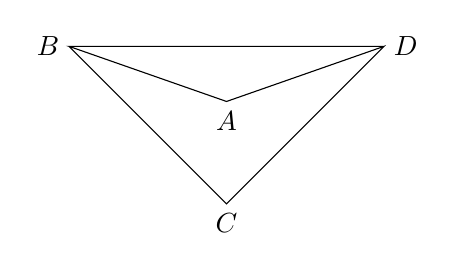
\begin{tikzpicture}
		\draw(0,0)node[left]{$B$}--(2,-2)node[below]{$C$}--(4,0)node[right]{$D$}--(2,-.7)node[below]{$A$}--(0,0)--(4,0);
	    \end{tikzpicture}
	\end{center}

	Demostración.-\; Dado que el triángulo $BCD$ es isósceles, entonces $C\widehat{B}D = B\widehat{D}C$. Cómo $C\widehat{B}D = D\widehat{B}A + \widehat{B}C$ y $B\widehat{D}C = B\widehat{D}A + A\widehat{D}C$ entonces: $$D\widehat{B}A + A\widehat{B}C = B\widehat{D}A + A\widehat{D}C$$ Cómo $D\widehat{B}A = B\widehat{D}A$ porque  $\triangle BDC$ es isósceles, entonces $A\widehat{B}C = A\widehat{D}C$. Y por el criterio $LAL$ tenemos que $\triangle BAC = \triangle ADC$ lo que implica que $AC$ es bisectriz.\\\\

	%--------------------12.
	\item Justifique el siguiente procedimiento para determinar el punto medio de un segmento. $“$Sea AB un segmento. Con un compás centrado en $A$, construya un círculo de radio $AB$. Construya otro círculo del mismo radio y centro en $B$. Estos dos círculos se intersectan en dos puntos. Trace la recta que une estos puntos. La intersección de esta recta con el segmento AB será el punto medio de $AB$.$”$

	\begin{center}
	    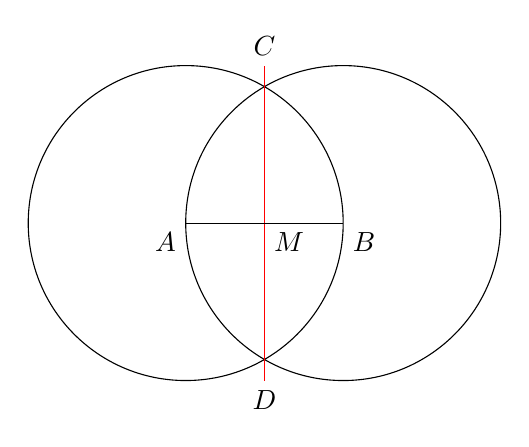
\begin{tikzpicture}
		\draw(0,0) circle (2cm)node[below left]{$A$};
		\draw(2,0) circle (2cm)node[below right]{$B$};
		\draw[red](1,-2)--(1,2);
		\draw(0,0)--(2,0);
		\draw(1,0)node[below right]{$M$};
		\draw(1,2)node[above]{$C$};
		\draw(1,-2)node[below]{$D$};
	    \end{tikzpicture}
	\end{center}

	Respuesta.- Donde notamos que $CB = CA = BD = DA = \; radio$. Entonces $\triangle CBA = \triangle BDA$ y $\triangle CAD = \triangle CBD$. Según los criterios de coincidencia $\triangle CBM = \triangle CMA = \triangle BDM = \triangle MDA$, entonces $BM = MA$ y la línea $r$ interseca el segmento $BA$ en el punto medio.\\\\

	%--------------------13.
	\item ¿En la construcción anterior, es realmente necesario que los dos círculos tengan radio $\overbrace{AB}$?\\\\
	Respuesta.-\;

	%--------------------14.
	\item Muestre que en la construcción descrita en el problema $12$, la recta que determina el punto medio de $AB$ es perpendicular a $AB$.\\\\
	Demostración.-\;

	%--------------------15.
	\item Utilice la idea de la construcción descrita en el problema $12$ y proponga un método de construcción de una perpendicular a una recta dada pasando por un punto de esta recta.\\\\
	Respuesta.-\;

	%--------------------16.
	\item En la figura, se tiene $AD=DE$, $\widehat{A}=D\widehat{E}C$ y $A\widehat{D}E=B\widehat{D}C$. Muestre que los triángulos $ADB$ y $EDC$ son congruentes.
	
	\begin{center}
	    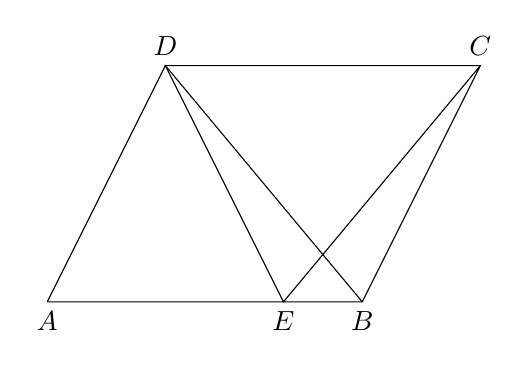
\begin{tikzpicture}
		\draw(0,0)node[below]{$A$}--(4,0)node[below]{$B$}--(5.5,3)node[above]{$C$}--(1.5,3)node[above]{$D$}--(3,0)node[below]{$E$}--(5.5,3);
		\draw(4,0)--(1.5,3)--(0,0);
	    \end{tikzpicture}
	\end{center}
	Demostración.-\; Como $AD = DE$, tenemos un triángulo isósceles. De esta forma, los ángulos de la base son congruentes. $\widehat{E} = \widehat{A}$. $DE$ es común para los dos triángulos $ADE$ y $DEC$, que también es un triángulo isósceles. $AD = DE$ son congruentes como se indica por tanto, los ángulos $A$ y $D$ son congruentes y sus bases son iguales. $AD = DE$. Asimismo, los ángulos $A$ y $E$ son congruentes, $D$ y $E$ son congruentes y $A$  $B$ son congruentes. Por la proporcionalidad de las bases y la congruencia de los ángulos, podemos decir que los triángulos $ADB$ y $EDC$ son congruentes.\\\\

	%-------------------17.
	\item Mostrar que en un triángulo isósceles $ABC$, con base $BC$, la bisectriz a la base es una mediana.\\\\
	Demostración.-\;

    \end{enumerate}
